\section{ Motivation}

As a result of increasing human population and habitat loss, human-wildlife conflicts have become increasingly common in recent decades\cite{philip-wildlife}.
According to the organisation The World Wide Fund for Nature (WWF), human-wildlife conflicts are defined as: "any interaction between humans and wild animals, that results in negative impacts on human social, economic or cultural life, on the conservation of wildlife populations, or on the environment"\cite{conflict-manual}.
These conflicts range from mostly harmless, non-violent contacts, such as sightings of wildlife animals in urban areas, to the destruction of crops and infrastructure, killing of livestock, and, in the worst cases, loss of human lives.
In more severe cases these conflicts end in defensive or retaliatory killings of wild animals, which can drive an already endangered species to extinction.

Polar bears, tigers, and elephants are generally considered to be the most problematic \cite{philip-wildlife}.
In the Arctic, as a consequence of the reduction of their natural habitat, polar bears are drawn to human settlements and food dumps while searching for food\cite{wildlabs-polarbears}.
Unexpected encounters can become deadly for both sides.
As wide-ranging animals, tigers need large areas where they can roam, hunt, and breed\cite{wildlabs-tigers}.
When their natural prey population is depleted, they often turn their attention to poorly protected livestock. 
Their attacks often have economic, social, and psychological consequences.
According to WILDLABS, tigers killed 101 people between the years 2013 and 2016, in India alone\cite{wildlabs-tigers}.

As herbivores, elephants might be seen as less problematic when compared to polar bears or tigers, but this assumption could not be further from the truth.
Although exact numbers vary between sources, casualties from Human-Elephant Conflicts (HEC) are much higher compared to conflicts involving polar bears or tigers.
According to WILDLABS, an average of 400 people and 100 elephants are killed every year in India\cite{wildlabs-elephants}. 
The leading cause of death of elephants is electrocution (by electric fences, unprotected power lines), followed by train accidents, poaching, and poisoning\cite{cause-of-death}.
Reasons for HEC are similar to the conflicts with polar bears and tigers.
Their habitat is shrunk continuously and replaced with crop fields and plantations.
As their food options decrease, surrounding agricultural landscapes become inviting.  
Various HECs can be seen in figure \ref{various_hec}.

\begin{figure}[ht]
    \begin{subfigure}{0.5\textwidth}
        \centering
        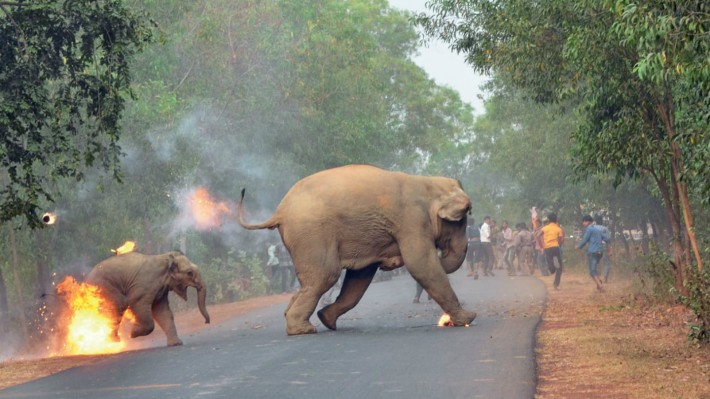
\includegraphics[width=1.0\linewidth, height=5cm]{hec_a.jpg} 
    \end{subfigure}
    \begin{subfigure}{0.5\textwidth}
        \centering
        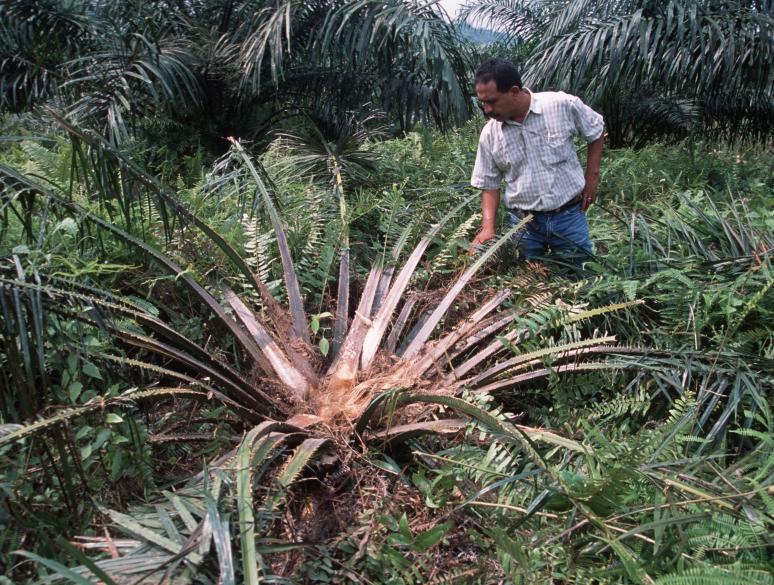
\includegraphics[width=1.0\linewidth, height=5cm]{hec_b.jpg} 
    \end{subfigure}
    %
    \begin{subfigure}{0.5\textwidth}
        \centering
        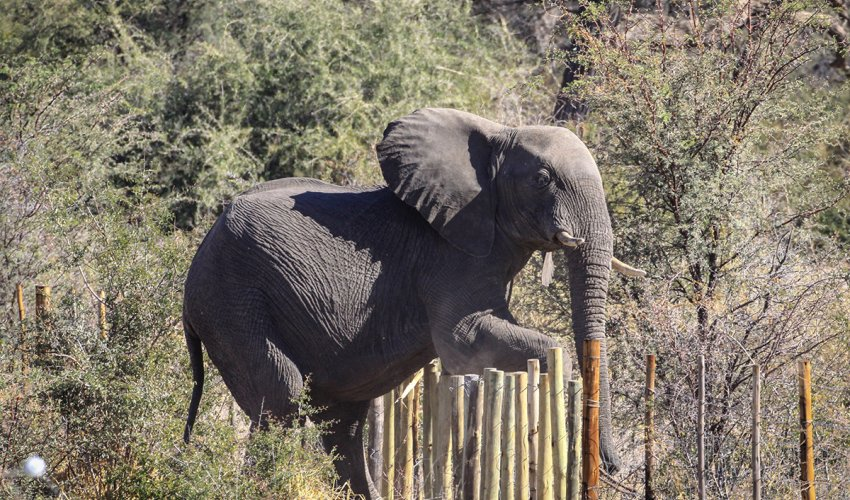
\includegraphics[width=1.0\linewidth, height=5cm]{hec_c.jpg} 
    \end{subfigure}
    \begin{subfigure}{0.5\textwidth}
        \centering
        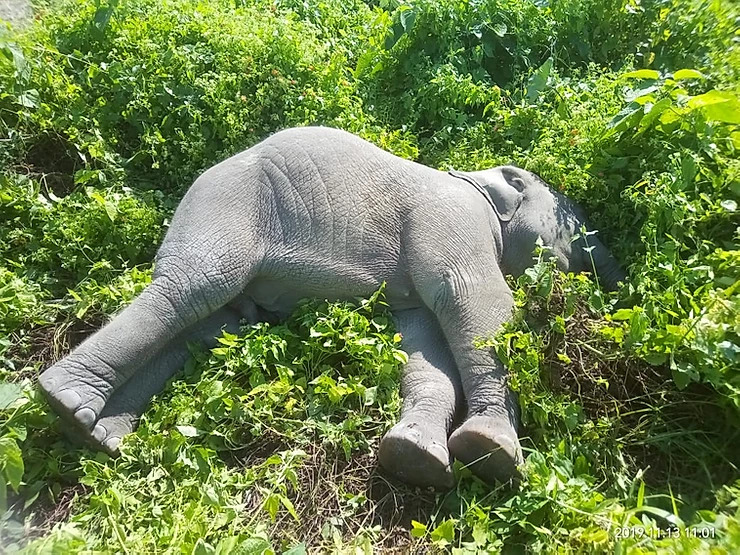
\includegraphics[width=1.0\linewidth, height=5cm]{hec_d.jpg} 
    \end{subfigure}
\caption[Various Human-Elephant Conflicts.] {Various Human-Elephant Conflicts. Top left: two elephants running from a mob hurling flaming tar balls, top-right: palm plantation owner inspecting damage done by elephants to the crops, bottom-left: an elephant crossing the protective barrier, bottom-right: An elephant that died because of HEC. Image sources:\cite{wildlabs-elephants}\cite{econe_image}\cite{save_our_species_image}\cite{the_week_image}}
    \label{various_hec}
\end{figure}

One of the HEC hotspots is in the Sonitpur District, Assam Province, India. 
In a 5300 km\textsuperscript{2} large area around 200,000 people and 200 elephants share the same space\cite{wildlabs-elephants}.
Elephants often venture into paddy fields which represent livelihood for local communities.
A single elephant can quickly trample fields of rice crops in a few hours, causing big financial problems to already impoverished farmers\cite{wildlabs-elephants}.

Several measures have been taken to minimise HEC: Electrical fences, watch towers, trenches, chilli-based deterrents, regular patrols, usage of trained captive elephants and camera traps with motion sensors.

Although the above mentioned measures function to some degree, they are not effective enough, since they are unreliable, or come into effect when the damage has already been done\cite{wildlabs}. 

\section{ Early warning system}\label{early_detection_system}

One important component of minimizing Human-Elephant Conflicts is a reliable early warning system. 
A system capable of detecting the presence of nearby elephants would warn nearby communities and give them enough time to prepare and respond non-violently.
The same kind of system would also provide information about common elephant paths, thus giving farmers knowledge on how to construct and place their fences better to minimise HEC.
The system (Figure \ref{early_detection_system_diagram}) should consist of several small, deployed devices with mounted cameras that will detect elephants, and one server which will aggregate alerts and forward them to mobile phones and computers, where the local community will see them.

\begin{figure}[ht]
        \centering
        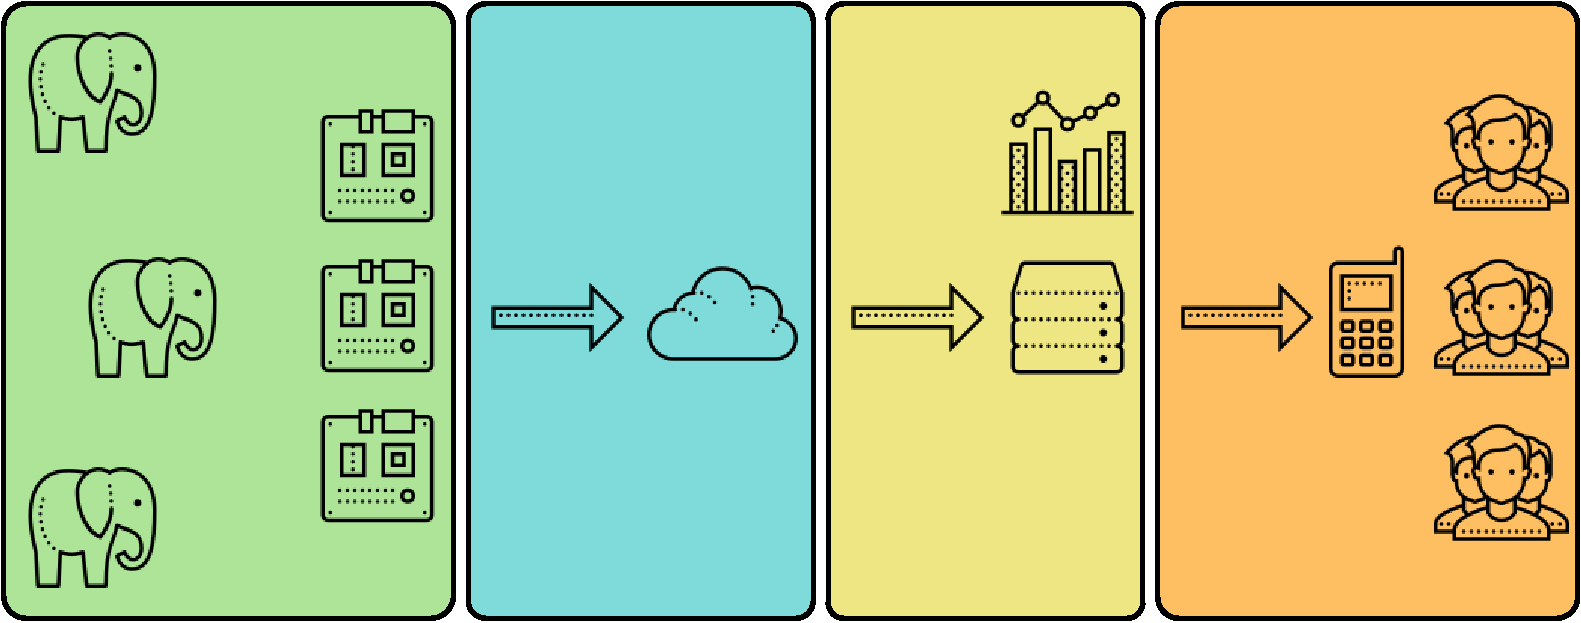
\includegraphics[width=1.0\linewidth]{early_detection_system.pdf} 
        \caption[Diagram of an early warning system.]{Diagram of an early warning system. Icons source:\cite{icons}}
        \label{early_detection_system_diagram}
\end{figure}

Although most of the villages in the Sonitpur district have access to cell phones and the internet, the connectivity can be unreliable\cite{wildlabs-elephants}. 
Furthermore, devices will be placed quite far from the main server, which makes sending a large amount of data a problem. 
This limits the choice of wireless networks to long range, low bandwidth technologies.
It is, therefore, preferable that elephant detection is done on deployed devices, and only results (which can be few bytes big) are sent over some radio network to the main server.
Deployed devices will be placed in forests, fields, with no access to electricity, therefore, they need to be battery powered.
Low maintenance of deployed devices is a desirable quality, which means that they should be functional for longer periods without any human interactions.
To achieve that with a limited power source, they should be energy efficient, equipped with solar panels, and a low power radio.
Devices should spend most of their time in sleep mode, conserving energy, only waking up to take a photo, processing it, and sending results to the main server.
A thermal camera is needed, as most of the Human-Elephant Conflicts happen during the night\cite{wildlabs-elephants}.

Elephant recognition can be done with the help of a convolutional neural network (CNN) running inference on a microcontroller. 
Making this possible and evaluating the solution is the focus of this master's thesis.


\section{ IRNAS and the Arribada Initiative}\label{arribada_init}

The system described above is currently in development at IRNAS in the collaboration with Arribada Initiative.
The Slovenia based Institute IRNAS offers a complete development service, starting with an idea on paper and ending with a finished product. 
Its previous projects cover a wide range of different fields, from free space optical systems, bio-printing, to Internet of things (IoT) solutions that cover various industrial and nature conservative use cases.
The Arribada Initiative is a London based team, that uses open source solutions for purposes of nature conservation.
As the winner of WWF and WILDLABS Human Wildlife Conflict Tech Challenge\cite{wildlabs-winners}, Arribada received funding to develop an early warning system.
They spent some time in Assam, India, where they tested a proof-of-concept design\cite{arribada-assam}.
They decided on devices with thermal cameras, as Human-Elephant conflicts often happen during the night.
The sensor of choice was an FLIR Lepton 2.5 and/or 3.5.
They also created a large dataset of elephant images while filming elephants in Whipsnade Zoo in the United Kingdom. 
This dataset will be important for training the Neural Network, and it will be discussed in Section\ref{exploring_dataset}.
To create a final embedded system with on device Machine Learning, Arribada chose to work with IRNAS.


\section{ Reasoning for the Machine Learning approach}

Today Machine Learning (ML) is present in many products that we use on a daily basis.
It can be found in email spam detection, recommendation algorithms on Facebook and YouTube, speech recognition on smartphones and medical applications.
ML can help us solve problems that are hard to solve by conventional methods.
For example, to develop an email spam detector, a programmer would have write a program that would scan the content of an email while checking for the common words and phrases that appear in spam emails and flag the email as spam if they would be found.
This would take several iterative cycles of writing the rules, evaluating the solution and analysing the possible mistakes. 
Even if a possible deterministic solution would be made, it would not stand the test of time, as new forms of spam emails would emerge, tricking the system.

Compare that to a Machine Learning approach. 
Given enough examples of spam and normal emails, we can train an ML algorithm and let it to discover by itself the rules that mandate what is a spam and what is a normal email.
The program would be much smaller compared to the one made by the conventional approach. 
After the program is launched into the real world, we can use it to store new data and relearn, thus always adapting to new changes.
This process can be automated.

Same parallels can be drawn to recognising elephants from thermal images.
It is an impossible task to write a deterministic algorithm that could identify an elephant successfully from an image and not confuse it for a human or livestock. 
Using an ML approach we can train the algorithm on a image dataset and let it figure out the connections between the images and correct labels. 


\subsection{ Implementation of Machine Learning algorithms}

Since ML algorithms are at their core normal math operations, they can be implemented (although maybe not efficiently) in any programming language and on any hardware platform from scratch.
However, to avoid reinventing the wheel and wasting the time on algorithm optimisation, it is more logical to use one of ML frameworks.
Frameworks such as scikit-learn, Keras, Caffe and TensorFlow enable programmers to write application code in a high level language such as Python, which, at run time, translates to efficient C/C++ code. 
These frameworks take away low-level details of ML algorithms, enabling programmers to deal only with application code and not its underlying implementation.

In several past years there has been a growing desire to expand ML applications to embedded devices.
Running ML algorithms directly on microcontrollers has benefits and challenges compared to running it on computers and servers.
These comparisons are described further in Section \ref{ml_on_embedded}.
There are several frameworks, proprietary and open-sourced, that can be used to develop ML applications on microcontrollers.
STMicroelectronics created X-CUBE-AI, a tool that converts the pre-trained model created by one of the various Deep Learning frameworks into an optimised library. 
X-CUBE-AI works only with STM32 microcontrollers, and is proprietary.
Another framework, TensorFlow Lite for microcontrollers, was created as an extension of TensorFlow Lite, which was used to develop ML models for mobile applications.
It provides converter tools and C++ implementations of common ML operations.
In 2019 another framework, \si{\micro}Tensor, was merged with TensorFlow Lite, providing it with support for an efficient CMSIS-NN library developed by ARM.

For this thesis we used TensorFlow Lite for microcontrollers.
It can be used with any family of microcontrollers, and is open-source, so we can study its internal code.


\subsection{ Edge Impulse}

Regardless of the many Ml frameworks on the market, companies that specialise in ML on embedded devices are scarce.
One of them is Edge Impulse, which is a recently founded company in San Jose, USA.
They provide users with an end to end web solution for developing ML applications for embedded devices.
Instead of designing and writing specific programs that deal with preprocessing of training data and creation and training of ML models, Edge Impulse does this automatically for their customers.
After the ML model is created and converted into an optimised format for embedded systems, customers get the immediate first approximation of how much RAM and FLASH memory the model will take and how fast it will run.
We can then run the model on the local machine, or deploy to a variety of different platforms, such as Arduino, STM32, OpenMV, Zeyphr and others.

Their solution will be used as a benchmark for our work with TensorFlow Lite.


\section{ Objective}\label{objective}

The objective of this Master's thesis is to evaluate the feasibility of  animals, especially elephants, from thermal images, with Machine Learning algorithms, running directly on a microcontroller.

The objective of this Master's thesis is to design and build a system capable of detecting an elephant with the help of Machine Learning algorithms in the day or at night.
Detection of an elephant needs to be reported over a wireless network to an application server.

For that we will:

\begin{itemize}
    \item Train a Neural Network model capable of classifying elephants, humans and other animals from thermal images.
    \item Optimise Neural Network model for on device inference.
    \item Implement on device inference on an STM32 microcontroller using TensorFlow Lite.
    \item Compare the performance of our implementation against the Edge Impulse implementation.
    \item Build a system around the STM32 microcontroller with a thermal camera and wireless network support.
    \item Profile power consumption of the built system.
    \item Establish system requirements for different ML applications.
\end{itemize}


\section{ Master's thesis outline}

This chapter provided an overview of motivation and the companies involved, some reasoning for choosing the Machine Learning approach and the objectives of this thesis.
Chapter 2 provides a theoretical description of the system building blocks. Machine Learning, Neural Networks, thermal cameras, TensorFlow Lite, and others topics are discussed there.
Chapter 3 revolves around the design of an image classification Neural Network model.
Chapter 4 describes the design and implementation of an early warning system, from the hardware, firmware and software points of view.
In Chapter 5 we describe the measurement procedure and results.
Chapter 6 presents our findings, describes the limitations of our project, and suggest paths for further research.

